\section{Diskussion}
\label{sec:Diskussion}
Die zum Anfang zu überprüfende Bragg Bedingung wurde ausreichend gut verifiziert. So weicht der experimentelle Wert des Glanzwinkels
nur um
\begin{align*}
p_\text{Bragg} = \frac{13,75\,°}{14,00\,°} - 1 = 1,79\,\%
\end{align*}
ab. Ebenfalls gut wurde die minimale Wellenlänge und damit auch die maximale Energie der Photonen sehr genau gemessen. Die relative Abweichung
der Energie vom Literaturwert\cite{kent} ist mit
\begin{align*}
p_\text{E} = \frac{36\,\si{\kilo\electronvolt}}{35\,\si{\kilo\electronvolt}} - 1 = 2,86\,\%
\end{align*}
sehr gering.
Das Auflösungsvermögen mit:
\begin{align*}
\Delta E = (\num{0.170 +- 0.040})\,\si{\kilo\electronvolt}
\end{align*}
lässt sich leider nicht mit einem Literaturwert vergleichen. Da das Röntgenemissionsspektrum eine statistische Verteilung darstellt, können so bei einer recht kleinen Integrationszeit
von $\Delta t = 5\,\si{\second}$ immer leichte Fehler entstehen. Es müsste also für jeden eingestellten Winkel ein längeres Zeitintervall betrachtet werden, um so einen genaueren
Wert über diese Größe bestimmen zu können. Aber dadurch, dass das Auflösungsvermögen recht gering ist, wird davon ausgegangen, dass es sich hierbei doch um eine gelungene Näherung
der Halbwertsbreite handelt.
Die im zweiten Teil der Auswertung berechneten Energien der Elemente mit Ordnungszahlen $30 \leq Z \leq 50$ werden ebenfalls mit den Literaturwerten\cite{kent2} verglichen. Der Vergleich mit den
Abweichungen befindet sich in Tabelle \ref{tab:vergleich}.
\begin{table}[H]
  \centering
  \caption{Vergleich zwischen den experimentellen Energien mit denen der Theoretischen.}
  \label{tab:vergleich}
\begin{tabular}{c c c c}
  \toprule
Element & $E_\text{K, exp}\:/\: \si{\kilo\electronvolt}$ & $E_\text{K, lit}\:/\: \si{\kilo\electronvolt}$ & rel. Abweichung $/\:\%$ \\
\midrule
Zink & 9,651 & 9,669 & 0,19\\
Brom & 13,381 & 13,484 & 0,76\\
Strontium & 15,710 & 16,115 & 2,51\\
Zirkonium & 17,727 & 18,008 & 1,56\\
\bottomrule
\end{tabular}
\end{table}
\noindent Auch hier fällt auf, dass die gemessenen Werte nah an den Wert aus der Literatur liegen.
Die mit der Ausgleichsreichnung berechnete Rydbergenergie weicht auch nur gering vom Literaturwert\cite{kent} ab.
Die relative Abweichung liegt hierbei bei:
\begin{align*}
p_\text{ryd} = \frac{12,0\,\si{\electronvolt}}{13,61\,\si{\electronvolt}} -1 = \num{11,83}\,\%.
\end{align*}
Die zum Schluss untersuchte $K_2$- und $K_3$-Linie des Quecksilbers Absorptionsspektrums weist ebenfalls nur geringe Messabweichungen auf. Der Vergleich hierfür wird erneut mit Literaturwerten\cite{kent2}
durchgeführt und befindet sich in Tabelle \ref{tab:vergleich2}.
\begin{table}[H]
  \centering
  \caption{Vergleich zwischen den experimentellen Energien mit denen der Theoretischen.}
  \label{tab:vergleich2}
\begin{tabular}{c c c c}
  \toprule
$L$-Linie & $E_\text{L, exp}\:/\: \si{\kilo\electronvolt}$ & $E_\text{K, lit}\:/\: \si{\kilo\electronvolt}$ & rel. Abweichung $/\:\%$ \\
\midrule
$L_2$ & 14,222 & 14,217 & \num{0,04} \\
$L_3$ & 12,131 & 12,292 & \num{1,31} \\
\bottomrule
\end{tabular}
\end{table}
\noindent Zum Schluss lässt sich zusammenfassen, dass trotz der anfänglichen Bedenken über die statistische Verteilung der Röntgen Emissions- und Absorptionsspektren, die Messreihe nur sehr geringe
Abweichungen vorweist.

\section{Anhang}
Im Anhang befinden sich die erstellten Graphen.
\begin{figure}[H]
  \centering
  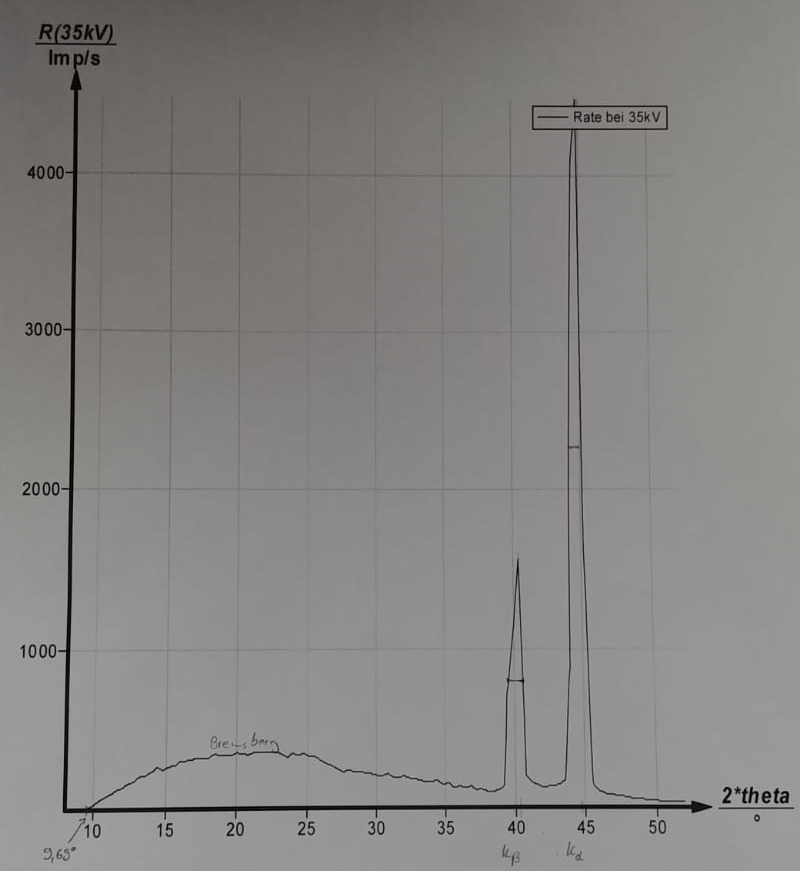
\includegraphics{emission.png}
  \caption{Das Emissionsspektrum einer Cu-Röhre mit Bremsberg, $K_\text{beta}$- und $K_\text{alpha}$-Kante.}
  \label{fig:plot}
\end{figure}

\begin{figure}[H]
  \centering
  \includegraphics{zink.png}
  \caption{Graphische Darstellung des Absorptionsspektrums von Zink mit eingezeichneter K-Kante.}
  \label{fig:plot}
\end{figure}

\begin{figure}[H]
  \centering
  \includegraphics{brom.png}
  \caption{Graphische Darstellung des Absorptionsspektrums von Brom mit eingezeichneter K-Kante.}
  \label{fig:plot}
\end{figure}

\begin{figure}[H]
  \centering
  \includegraphics{strontium.png}
  \caption{Graphische Darstellung des Absorptionsspektrums von Strontium mit eingezeichneter K-Kante.}
  \label{fig:plot}
\end{figure}

\begin{figure}[H]
  \centering
  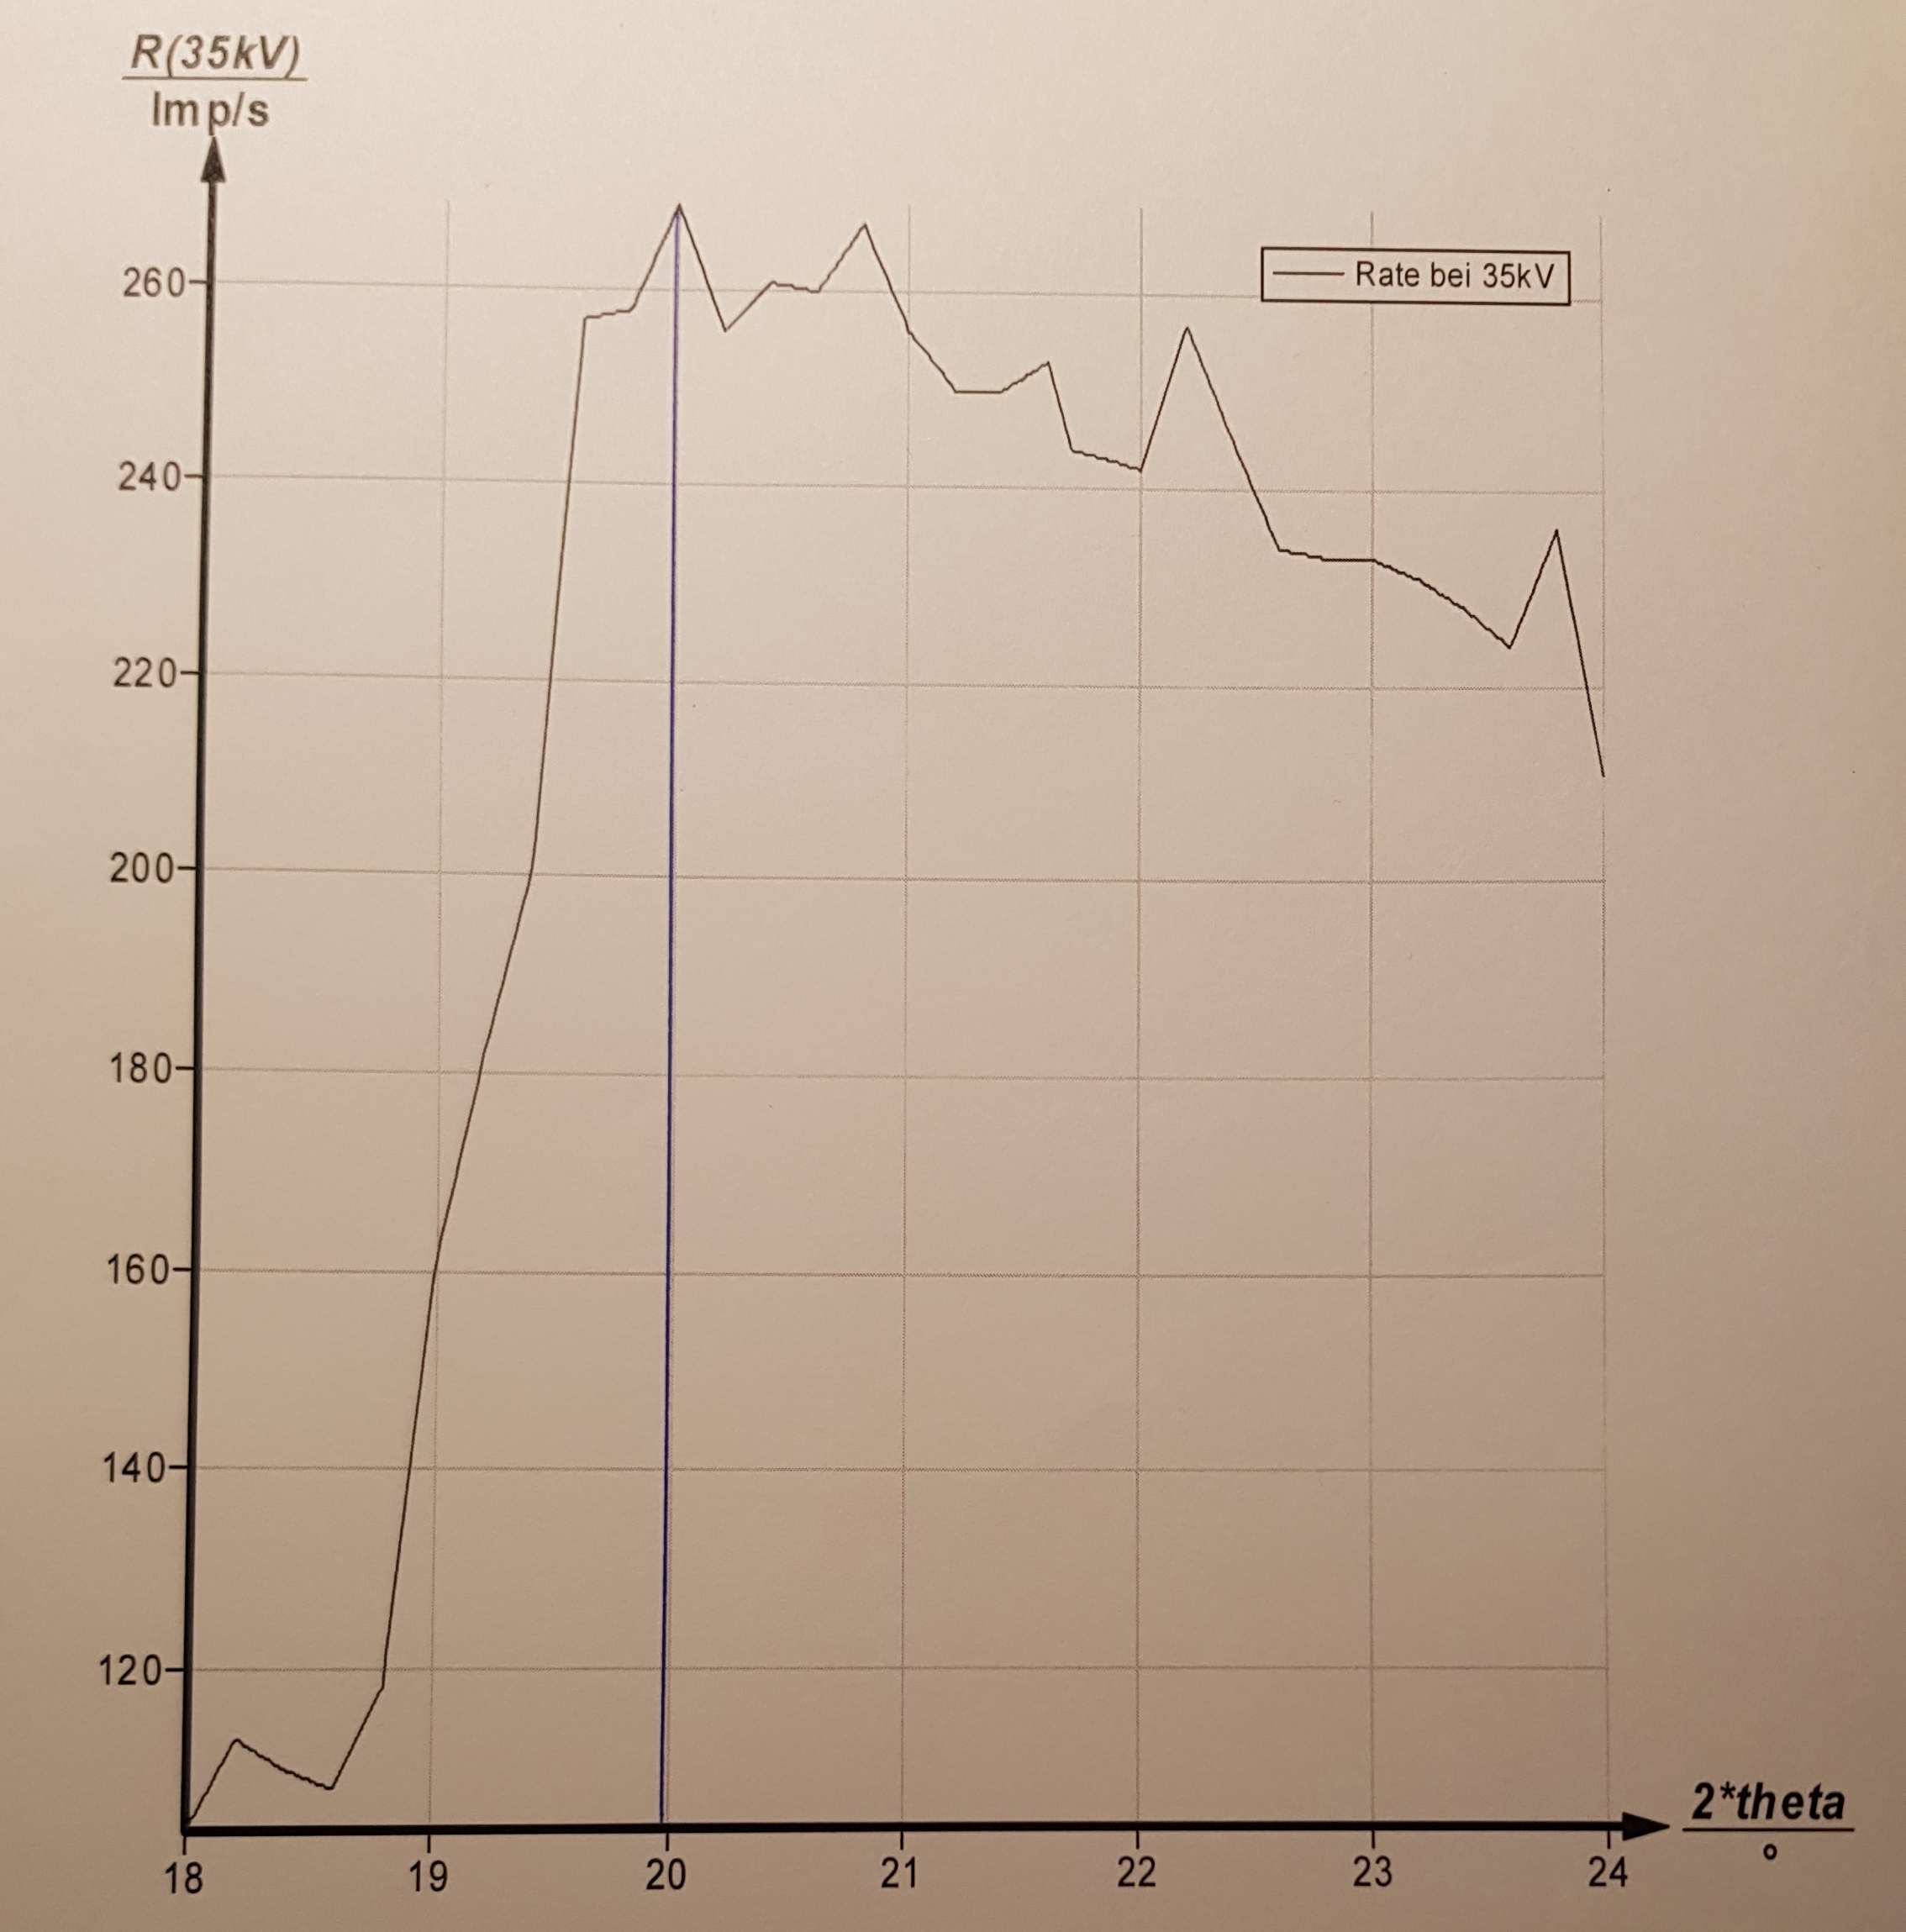
\includegraphics{zirkonium.png}
  \caption{Graphische Darstellung des Absorptionsspektrums von Zirkonium mit eingezeichneter K-Kante.}
  \label{fig:plot}
\end{figure}

\begin{figure}[H]
  \centering
  \includegraphics{hg.png}
  \caption{Graphische Darstellung des Absorptionsspektrums von Quecksilber mit eingezeichneter $L_\text{3}$- und $L_\text{2}$-Kante.}
  \label{fig:plot}
\end{figure}